\section{Comparaison avec la photo plus
lumineuse}\label{comparaison-avec-la-photo-plus-lumineuse}

\begin{figure}[htbp]
\centering
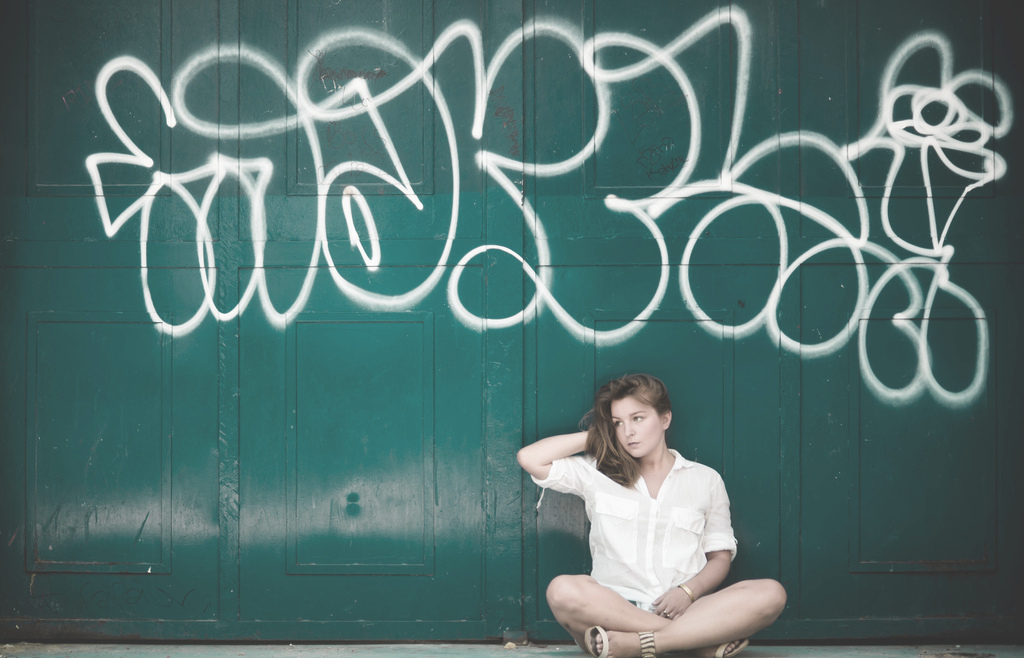
\includegraphics{../../photos/lumineux.jpg}
\caption{Photo plus lumineuse}
\end{figure}

\begin{table}[htbp]
\centering
\begin{tabular}{llr}
\bfseries Formes (\%)&
\bfseries Bhattacharyya (\%)%
\DTLforeach*[\DTLiseq{\fichier}{photos/lumineux.jpg}]{valeurs}{%
\fichier=Fichier, \formes=Formes,\bhatta=Bhattacharyya, \hue=Hue, \saturation=Saturation, \value=Value}{%
\\
\formes & \bhatta}
\end{tabular}
\end{table}


On observe que la luminosité ajoutée à notre photo d'origine est suffisante
pour donner une différence colorimétrique de $51.53 \%$ par la distance de
Bhattacharyya. Par contre, le changement de luminosité ne change que très peu
les contours des formes, seulement $12.43 \%$ de différence après application
du filtre de Sobel.
